\chapter{Conclusion}
\label{chap:conclusion}

\newpage
{\footnotesize \hypersetup{linkcolor=black}
\minitoc}

\section{What are you hiding from me? A review of data resolution, expectations and fears, and realistic counter-measures in visualization.}
\subsection{Introduction and Motivation}
With big data rapidly becoming a standard within the field, Many have been wondering what they must do to represent everything given to them. At the EuroVis conference 2017, in his capstone presentation, Helwig Hauser brings up the idea of the human vision bandwidth to discuss the brain's capability to interpret information. Hauser states that color and transparency are only temporary solutions and may not be useful when our data sets are 10 orders of magnitude larger than current data sets \cite{hauser2019from}. We review this while looking at Schneiderman's information seeking mantra, \emph{" Overview first, zoom and filter, then details-on-demand"}, specifically the first step, gaining an overview of the entire collection \cite{shneiderman1996eyes}. If we can no longer use even color, how can we enable a full overview in one view? The answer may be simpler than expected, and that is to reduce the resolution of data to present.

We suggest \textit{low resolution} visualization. Low resolution visualization describes a representation of a visualization with a reduced level of detail. We believe that low resolution should be used to present an overview of the data while (a) still presenting an overview of the underlying data (b) presenting close approximations of the underlying data, and (c) still allowing the user to clearly understand where and how zooming and filtering will be useful. However, implementing a low-resolution view can be taken negatively. By creating approximations of data, values end up being skewed, and when values are skewed people can gather false insight and false results. This issue is a well-known problem even outside of the visualization landscape. The Modifiable Areal Unit Problem (MAUP) looks at how aggregating values appointed to a 2D space can vastly change the results depending on how which areas you select \cite{openshaw1984modifiable}.
We also consider that many people assume that something unseen, has been decided to be unseen.

We believe that low resolution is a strong concept that could improve any visualization tool and techniques to be used as clutter reduction for visualization techniques that would find difficulty with common reduction techniques.  We look into why low-resolution visualization should not be considered an issue, and preferably a useful tool to avoid cognitive overload. We also discuss common negative sentiment and ways to address issues that may be coupled with the idea.

%\subsection{Background}
\subsection{Cognitive Perception}
Perception is a large research area within visualization and is a leading consideration when designing software and visualization techniques. This large amount of work can be broken down into discrete categories such as color \cite{lee2013perceptually,heer2012color,szafir2018modeling}, size \cite{mcnabb2018when,borgo2014order,gramazio2014relation}, and motion \cite{simons2000current, driver1992motion, huber2005visualizing}. However, research on this topic can vary widely to consider the work comparing ease of perception against other techniques in the form of user studies \cite{rittschof1998learning} or guidelines on perceivability within specific topics \cite{kong2010perceptual}. When considering a visualization technqiue, recognizing perceivabilty as a key challenge can transform your software into a critical analyst tool.
\subsection{Hidden Data}
It is important to consider that there are many cases where data you visualize has already been transformed to reduce the complexity of data. If we look at census data, by law, before any data is made public, the data needs to be both anonymized annd grouped in order to protect the identity of persons both in name and location.
\subsection{Overview without full detail}
First, let's look at the information seeking mantra once more. An overview is considered the first step to understanding, and because of this, it is easy to consider this as everything needing to be represented. However, this is not the case. If everything could be understood from an overview, there would be no need for a user to ever zoom in or filter in the first place. If we compare the overview of a visualization to a modern shop, we must consider the overview as our initial view of a shop. If we conclude the outside of the shop is the overview, then our main point of emphasis is that displayed in the windows shop, while if we consider the interior, we are likely to see signs which lead us to where we would like to go. An overview should be considered a gateway to enable zooming and filtering.

In order to make sure that reducing the resolution does not affect exploration, we can use techniques to minimize the effects of aggregation. In this section, we discuss two key areas: resolution indication and uncertainty visualization.
\subsubsection*{Resolution Indication}
If area resolution differs across 2D space, it is important to visualize where resolution may lie. We can use visual design variables in order to depict where frequency of data may lie. Borgo et al.\ combine multiple visual encoding variables to present a table of visual channels including geometric, optical, topological and relational, and semantic channels \cite{borgo2013glyph}. Refer to Table \ref{tbl:visualchannels}. 

\begin{table}
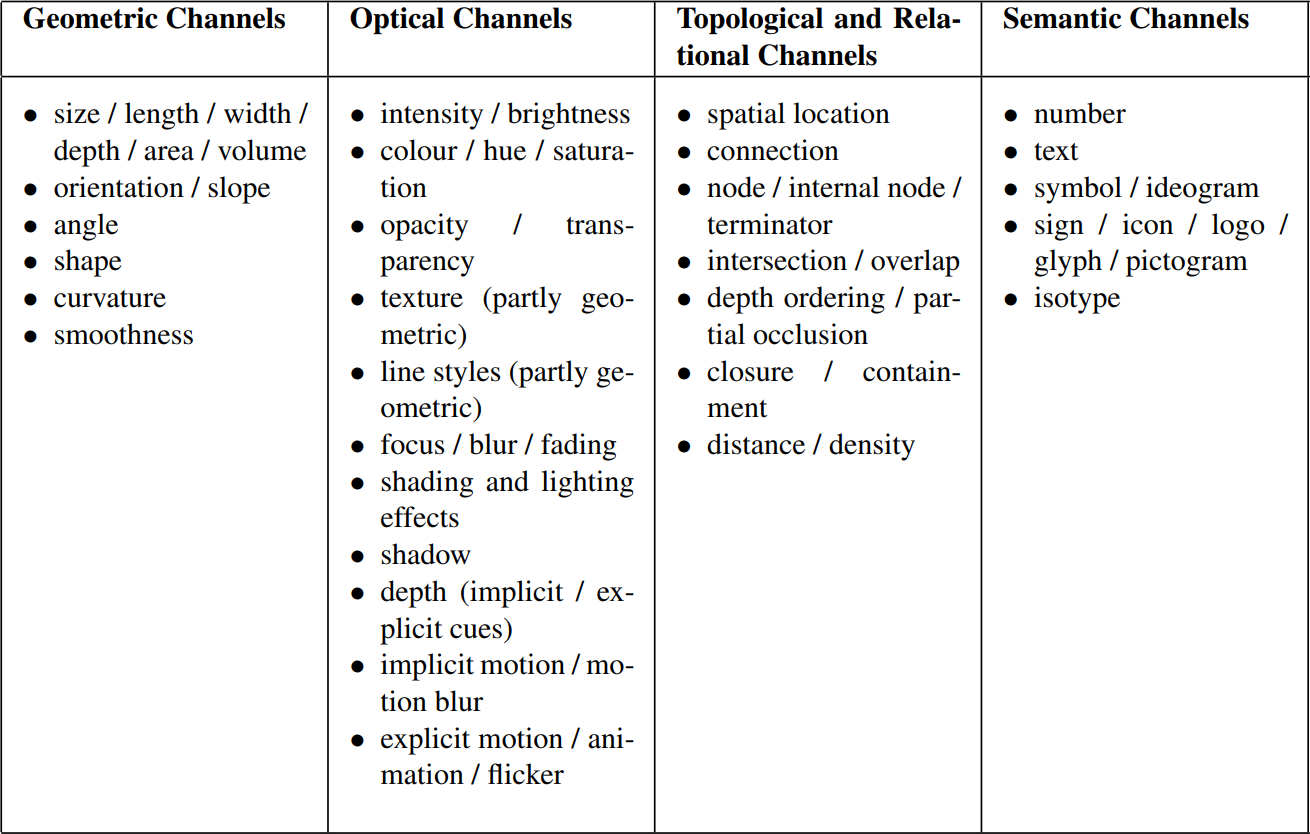
\includegraphics[width=1\linewidth]{images/ch7/visualchannels}
\caption{Visual channels presented by Borgo et al.\ \cite{borgo2013glyph}} \label{tbl:visualchannels}
\end{table}
\subsubsection*{Uncertainty Visualization}
Uncertainty visualization is a growing aspect of information visualization and applying these techniques towards low resolution is a logical process. Common uncertainty visualization normally uses visual mapping to deter close analysis, such as fuzzyness. However, when approaching uncertainty in low-resolution visualization, this normally sits in accordance with hidden indication and cause fuzzyness to be counter intuitive. We propose mitigating uncertainty by applying a matrix approach to your visual design of choice. If we use color as our visual channel to depict a the most common attribute of `A',`B', and `C', we can apply a bivariate color map to propose a value at the intersection of the highest selection and second highest selection. We could increase this by modelling a tri-variate color map that depicts the weighting of objects between the three values.
\subsection{Conclusion}
We discuss the concept of reducing data resolution to create low resolution visualization. We look at perception as well as the idea of hiding or anonymising data, and some considerations that need to be taken into account when creating a low resolutions visualization.
\section{Future Work}
During the process of the thesis, there were many avenues that the thesis could have followed. As such, we dedicate this section to discussing some of these ideas, as well as potential directions a subsequent candidate could follow during their PhD.

With regards to our literature review, We feel we have opened the doors to a range of potential survey papers under the SoS, or meta-survey branch. During the process of the thesis, other related surveys have been published \cite{alharbi2017molecular, alharbi2018sos, rees2019survey}. However, other avenues could be presented such as a Survey of Surveys for Geospatial, Scientific or Computer Graphics.

There are many avenues for future work for the merging algorithm presented in the thesis. Although we use real unit-areas, we would like to test with a broader range of choropleth data. The algorithm still has performance optimizations which could accelerate the speed even further, such as schematization \cite{barkowsky2000schematizing} which could be used to enable better optimization with the drawback of topological continuity being reduced. Other existing formats such as TopoJSON \cite{bostock2018topojson} look at reducing geometry redundancy and could be an excellent subsequent format for the procedure. We worked with 2D coordinate-spaces. A 3D coordinate space would be an exciting direction to take the algorithm and could open new applications for the process. The current termination method revolves around the idea of one area per contiguous region. Updates in the procedure could allow for more user control when it comes to stopping the merge procedure such as for categorical data where the most abstraction is introduced. Alternatively to this, a bi-variate color map could be implemented to display more accurate concordance of underlying values.  The algorithm potentially can apply to any data-sets with geometric boundaries and is open to new data structures. 

There are some limitations to the study we review in Chapter \ref{chap:userStudy}. We found boundary design to be a more significant factor for small sizes than anticipated. In the pilot study, we found that users had a much better accuracy overall, and comments were made about the area's color changing. This was actually due to the boundary's framing of the pixel, enhancing the perception of color based on the surrounding black contour. We try to control this as carefully as possible, however, this could be examined further in a follow-up study. We use real-world maps and areas. This means we do not control the aspect ratio of the areas, which may lead to more error in some situations such as narrow areas. This is an aspect that can be explored in an alternative study. T1 and T2 could hold a large amount of future research. For example, since we hold data about the location of the presented area and the color seeding, we could look back at what could have influenced the color decision for the area.

For our multivariate implementation in Chapter \ref{chap:MultivariateMaps}. At the moment, we use the raw derived centroid as a placement strategy. Although this removes a lot of density and occlusion, there is still some wasted space. We believe that by adding some overlap removal, we could use space more efficiently, while still avoiding any decoupling problems. Although we present some case studies, the algorithm could be more carefully compared to other glyph placement strategies with a user-study evaluation. We think the use of transitions was a great tool for understanding variation, but it is not always necessary. We feel that there are many avenues for exploring at multiple levels of detail. For example, directly zooming to a glyphs unit area extents may not need to represent zooming, to speed up exploration.

Now that we can improve performance on a second pass-through by saving build instructions to reduce the calculation of neighbor and boundaries, the next step would be to pipe multiple areas to be merged. This would allow the user to constrain area representation to the desired representation further. For example, if we look at the UK, OA's would only merge within their LSOA, and LSOA's would only merge within their MSOA's.
